\documentclass{standalone}

\usepackage[osf]{mathpazo}
\usepackage{microtype}

\newcommand\Direct{\textsc{Direct}}
\newcommand\CCD{CCD}
\newcommand\MDWS{MDWS}

\usepackage{tikz}
\usetikzlibrary
  {
    positioning,
    calc,
    intersections,
    backgrounds,
    fit,
    arrows,
    shapes.symbols,
    shapes.geometric,
  }
\tikzset
  {
    ->,
    >=latex',
    shorten >=.5pt,
    block/.style=
      {
        draw,
        fill=white,
        inner sep=.3em,
        rectangle,
        rounded corners=3pt,
        text height=1.3ex,
        text depth=.2ex,
        minimum size=3.6ex,
        align=center,
      },
    our code/.style={block, fill=blue!15},
    their code/.style={block, shape=ellipse},
    cloud/.style=
      {
        draw,
        shape=cloud,
        aspect=2,
        inner sep=1ex,
      },
    db/.style=
      {
        draw,
        fill=white,
        shape=cylinder,
        aspect=.3,
      },
    edge label/.style=
      {
        sloped,
        font=\tiny,
      },
    every pin/.style=
     {
       pin edge={red, -},
       red,
       font=\footnotesize,
     }
  }

\begin{document}

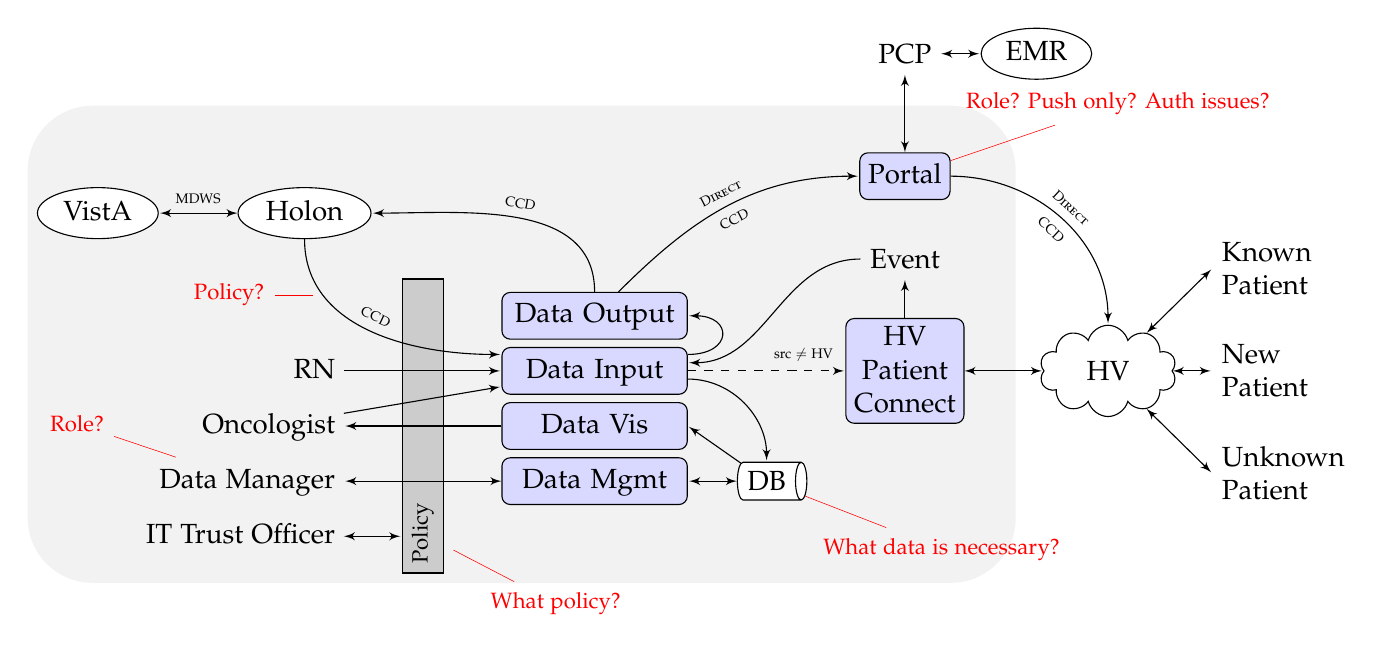
\begin{tikzpicture}
  \node[our code, text height=] (HVPC) {HV\\Patient\\Connect};
  \node[above=.5 of HVPC] (event) {Event};
  \node[our code, above=.5 of event, pin=above right:Role? Push only?
  Auth issues?] (portal) {Portal};
  \node[above=of portal] (pcp) {PCP};
  \node[their code, right=.5 of pcp] (emr) {EMR};

  \node[cloud, right=of HVPC] (HV) {HV};
  \begin{scope}[node distance=1.3, every node/.style={align=left}]
    \node[right=.5 of HV] (new) {New\\Patient};
    \node[above=of new.west, anchor=west] (known) {Known\\Patient};
    \node[below=of new.west, anchor=west] (unknown) {Unknown\\Patient};
  \end{scope}

  \begin{scope}
    [
      node distance=.7,
      every node/.style={our code, text width=13ex}
    ]
    \node[left=2 of HVPC, anchor=east] (input) {Data Input};
    \node[below=of input.east, anchor=east] (vis) {Data Vis};
    \node[below=of vis.east, anchor=east] (mgmt) {Data Mgmt};
    \node[above=of input.east, anchor=east] (output) {Data Output};
  \end{scope}

  \path (HVPC.west) -- coordinate (aux) (HVPC-|input.east);
  \node[db,pin={below right:What data is necessary?}] at (mgmt-|aux) (DB) {DB};

  \node
    [
      left=of vis,
      draw,
      rectangle,
      fill=black!20,
      rotate=90,
      anchor=center,
      font=\footnotesize,
      text width=3.5cm,
    ]
    (policy wall) {Policy};

  \node[pin={below right:What policy?}]
      at (policy wall.180 + 10) {};

  \begin{scope}[node distance=.7,
      every node/.style={our code, draw=none, fill=none},
  ]
    \node[left=2 of input.west] (RN) {RN};
    \node[below=of RN.east, anchor=east] (oncologist) {Oncologist};
    \node[below=of oncologist.east, anchor=east, pin={north west:Role?}]
    (data manager) {Data Manager};
    \node[below=of data manager.east, anchor=east] (trust officer) {IT Trust Officer};
  \end{scope}

  \begin{scope}[every node/.style={their code}]
    \node[above left=1 and 2.5 of output, anchor=center] (holon) {Holon};
    \node[left=of holon] (vista) {VistA};
  \end{scope}

  \begin{scope}[on background layer]
    \node
      [
        fill=gray!10,
        rounded corners=5ex,
        fit=(vista) (trust officer)
        (policy wall) ($(portal)!.5!(pcp)$)
        ($(HVPC)!.5!(HV)$)
      ] {};
  \end{scope}

  \draw (HVPC) -- (event);
  \draw[<->] (HVPC) -- (HV);
  \draw[<->] (HV) -- (known.west);
  \draw[<->] (HV) -- (new);
  \draw[<->] (HV) -- (unknown.west);

  \draw[out=0, in=90]
    (portal) to
    node[edge label, above] {\Direct}
    node[edge label, below] {\CCD}
    (HV);

  \draw[in=180]
    (output) to
    node[edge label, above] {\Direct}
    node[edge label, below] {\CCD}
    (portal);

  \draw[out=180, in=0] (event) to (input.5);
  \draw[dashed, out=0, in=180]
    (input) to
    node[edge label, above, near end] {src $\ne$ HV}
    (HVPC);

  \draw[out=0, in=0, looseness=3] (input.10) to (output);

  \draw (DB) -- (vis.east);
  \draw[<->] (DB) -- (mgmt.east);
  \draw[out=0, in=90] (input.-5) to (DB);

  \draw (RN) -- (input);
  \draw (oncologist) -- (input);
  \draw (vis) -- (oncologist);
  \draw[<->] (mgmt) -- (data manager);
  \draw[<->] (trust officer) -- (policy wall.north|-trust officer);

  \draw[out=90, in=0]
    (output) to node[edge label, above] {\CCD} (holon);
  \draw(holon) to [out=-90, in=-180]
    node[edge label, above] {\CCD}
    node[near start] (anchor) {}
    (input.170);
  \node[pin={left:Policy?}] at (anchor) {};
  \draw[<->] (holon) -- node[edge label, above] {\MDWS} (vista);

  \draw[<->] (portal) -- (pcp);
  \draw[<->] (pcp) -- (emr);
\end{tikzpicture}

\end{document}
